% !TeX root = ../FinalRepordCS.tex

\chapter{Project Outline and Methodology}

\section{Project Overview}
In this project, I am supposed to mainly implement each LoRa node hardware with a programmable Arduino shield and a Dragino’s LoRa expansion board for Arduino and then program the communication protocol with the Arduino IDE software with the LoRa KIT. Including the following:
\begin{itemize}
\item The implementation of LoRa nodes’ communication, such as signal sending and receiving, coding and decoding,
\item The extraction and analysis of the physical layer information between the communication process,
\item The implementation of the LoRa key generation and the test on it.
\end{itemize}

\section{Methodology}
\subsection{LoRa Physical Layer Emulation and Analyst}
Before the design and development in real vibe, the understanding and simulation of the LoRa physical layer could be significant since it has its characteristic, which is different from the standard communication protocol.
The LoRaPHY KIT is for LoRa Physical Protocol emulation\cite{10.1145/3546869}. Through this KIT, the payload of LoRa can be simulated, especially, and the encryption information can be analyzed and visualized before and after.
\begin{figure}
  \centering
  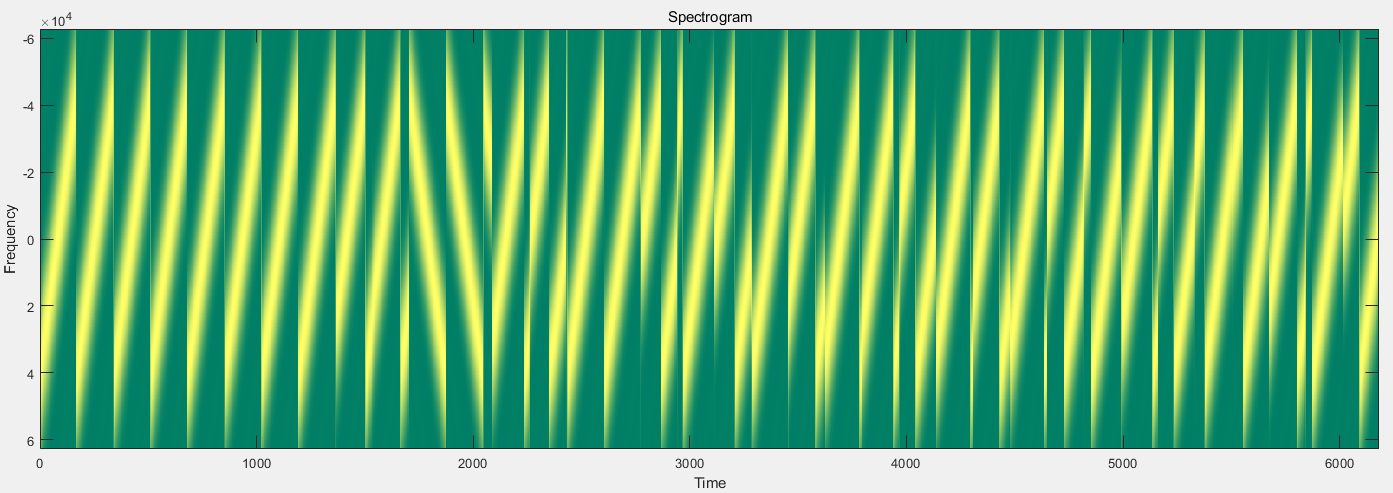
\includegraphics[width=1\linewidth]{fig3-1.png}
  \caption{A emulated LoRa physical layer payload of ‘[78 22 43 44 12]’}
  \label{fig:3-1}
\end{figure}

\subsection{Arduino Shield featuring LoRa technology}
In the realm of wireless communication, LoRa commonly employs the SX127x chipset, depicted in Fig 3-2 and manufactured by Semtech. An Arduino Shield, incorporating LoRa technology through an open-source library, serves as a practical manifestation. This shield facilitates the transmission of data over extensive distances at reduced data rates, harnessing ultra-long-range spread spectrum communication. Notably utilizing the Semtech SX1276/SX1278 chip, it is meticulously designed for applications in professional wireless sensor networks. These applications span diverse domains, including but not limited to irrigation systems, smart metering, smart cities, and building automation.

Furthermore, by leveraging the SX127x LoRa technique, the shield attains an impressive sensitivity exceeding -148dBm through the incorporation of a cost-effective crystal and bill of materials. This heightened sensitivity, complemented by the integrated +20 dBm power amplifier, results in an unparalleled link budget within the industry. This distinctive feature renders the shield exceptionally well-suited for applications demanding extended range or robust performance.

By using these components, the LoRa communication protocol can be well physically implemented and is a powerful and adaptable tool that can support the realization of the project.
\begin{figure}
  \centering
  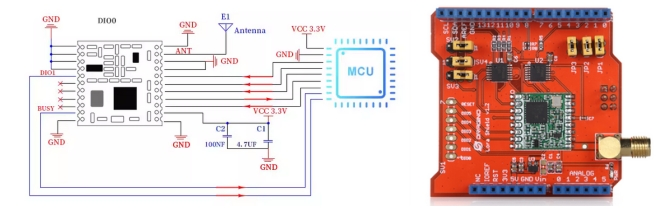
\includegraphics[width=1\linewidth]{fig3-2.png}
  \caption{The SX127x schematic diagram and physical representation}
  \label{fig:3-2}
\end{figure}

\subsection{Arduino’s UNO Programmable Board and IDE}
The Arduino Uno is a popular microcontroller board widely used in the maker and electronics communities for various projects and prototypes. Although the Arduino Uno itself does not possess native LoRa capabilities, it can be effectively employed as a control and interface unit to facilitate seamless integration with external LoRa modules or chipsets, shown as Fig 3-4. The integration process entails meticulous wiring connections between the Arduino Uno and the LoRa module, encompassing essential pins such as those for power (3.3V or 5V), ground (GND), and serial communication (TX and RX). Voltage levels are diligently considered to ensure compatibility between the Arduino Uno and the LoRa module. 
\begin{figure}
  \centering
  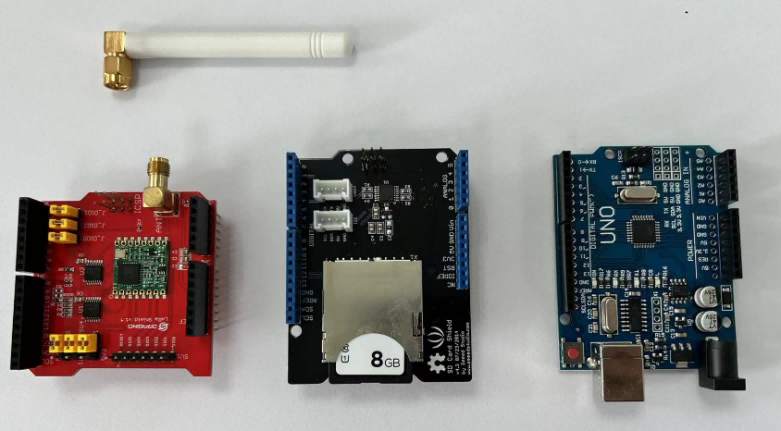
\includegraphics[width=0.6\linewidth]{fig3-3.png}
  \caption{The SX127x and Arduino’s UNO Programmable Board}
  \label{fig:3-3}
\end{figure}
In addition to the essential connections, supplementary connections, such as those related to module reset or configuration, may be required depending on the module's specifications. To facilitate effective communication with the LoRa module, the Arduino IDE is utilized. Relevant libraries that optimize interactions with the LoRa module are installed, ensuring the Arduino Uno is aligned with the specific requirements of the chosen module.

The subsequent phase entails the creation of Arduino code tailored to configure and orchestrate communication with the LoRa module. This code encompasses fundamental tasks such as module initialization, parameter configuration (e.g., frequency, spreading factor, bandwidth), and the transmission or reception of LoRa data packets. The intricacies of the code are contingent upon the precise LoRa module chosen and the intended application. Upon the completion of the code development, it is compiled and uploaded to the Arduino Uno via the ubiquitous USB interface, positioning the controller as a command and control center for the LoRa module.

By using this set of components, it is possible to effectively implement the logic for sending and receiving data between various LoRa nodes, as well as extracting features such as RSSI from the communication channel. Additionally, it enables the implementation of logic for physical layer encryption.


\subsection{Deep-in-Building and Outdoor Test}
The comprehensive evaluation of LoRa communication systems necessitates the execution of rigorous deep-in-building and outdoor tests, each designed to address distinct aspects of performance and coverage within varying environmental contexts.

The principal objective of the deep-in-building test for LoRa communication is to scrutinize the signal propagation characteristics within the intricate confines of interior structures, encompassing walls, floors, and architectural elements.

The outdoor test regimen for LoRa communication entails a meticulous assessment of the system's performance attributes in open-air or outdoor settings, characterized by the absence of indoor obstructions.
\begin{figure}
  \centering
  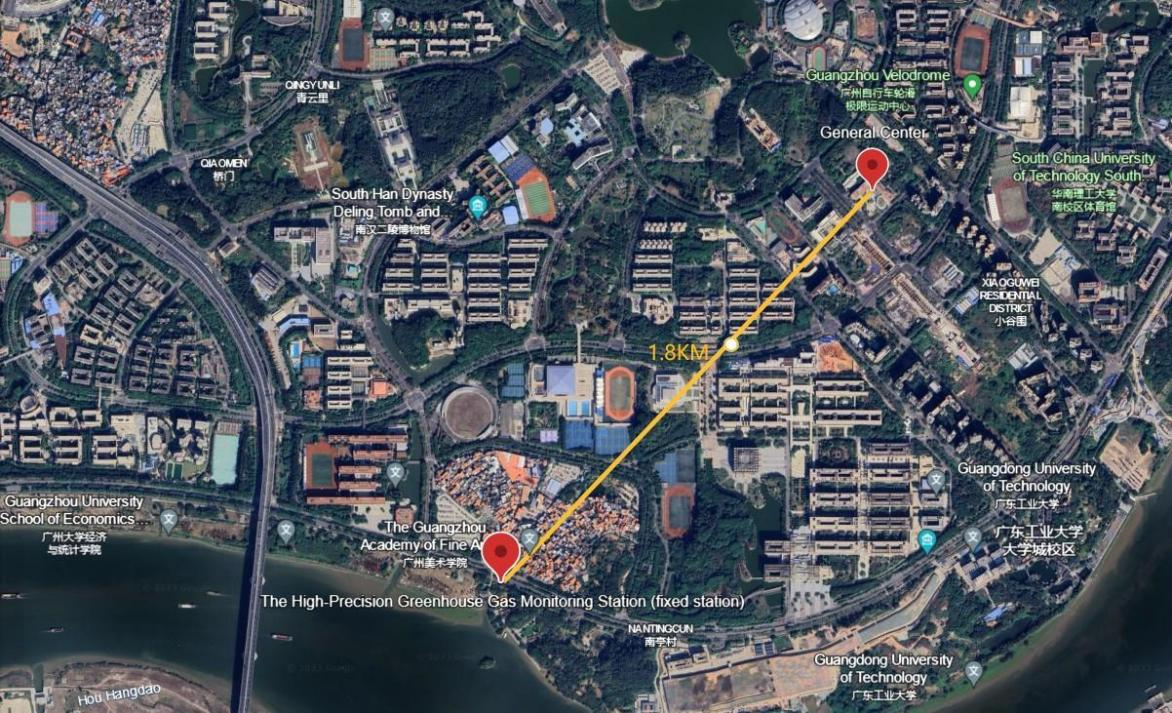
\includegraphics[width=1\linewidth]{fig3-4.png}
  \caption{Outdoor test between an fixed High-Precision Greenhouse Gas Monitoring Station and the General Center (1.8km)}
  \label{fig:3-4}
\end{figure}
At the same time, this testing plan is combined with a potential critical use case for LoRa technology in the field of environmental monitoring\cite{8515030}. Currently, most environmental monitoring data is transmitted using mobile networks, which can be costly and dependent on the infrastructure of telecommunication operators. In remote areas like the wilderness or deep in the mountains, there is often a lack of cellular signal coverage, even though environmental monitoring activities frequently need to be conducted in these areas. Therefore, this testing plan encompasses outdoor fixed monitoring stations, central monitoring facilities, and mobile monitoring stations for environmental monitoring. It is expected to effectively carry out a series of tests, including deep-in-building and outdoor tests.
\begin{figure}
  \centering
  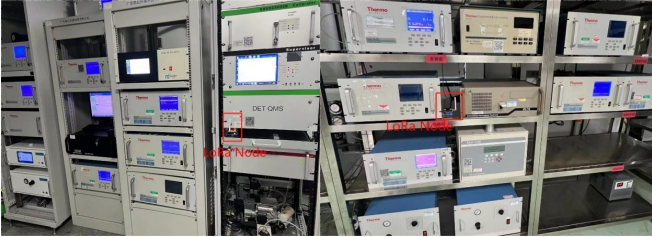
\includegraphics[width=1\linewidth]{fig3-5.png}
  \caption{Deep-In-Building Test at General Center}
  \label{fig:3-5}
\end{figure}

\subsection{Data Extraction and Analyst}
By testing in various scenarios, a series of test data can be obtained. The next step is to extract and preprocess the data. In particular, the analysis of feature data from the signals. Through the analysis of this data, we can understand the characteristics of LoRa signal features in different scenarios and under different electromagnetic background interferences.
Also, the Savitzky-Golay filter will be applied to the raw signal datasets. The filter is a commonly used technique in signal processing for smoothing or filtering noisy data, especially in the field of spectroscopy and chromatography. The primary goal of the Savitzky-Golay filter\cite{doi:10.1021/ac60214a047} is to remove noise from a signal while preserving the important features, such as peaks and valleys. It works by fitting a polynomial to a small window of data points and then using this polynomial to estimate the value of the central data point. This process is repeated for all data points, effectively smoothing the signal.
\begin{figure}
  \centering
  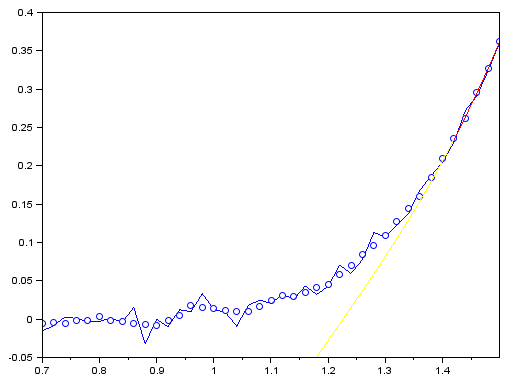
\includegraphics[width=0.5\linewidth]{fig3-6.png}
  \caption{Savitzky-Golay filter}
  \label{fig:3-6}
\end{figure}
After the data extraction and preprocessing, the analyst can begin to explore the characteristics of LoRa signal features in different scenarios and under different electromagnetic background interferences. This analysis will help to determine the optimal communication parameters and signal processing methods for specific applications. And Based on the results of these tests, the analyst can provide decision-makers with data-driven insights on how to optimize LoRa communication systems for different environmental contexts. This information is crucial for companies and organizations to make informed decisions about how to design, deploy, and maintain LoRa communication networks that are reliable and efficient for their specific applications.

\subsection{Physical Key Generation}
Physical layer key generation is a method for generating a shared secret key between wireless devices by exploiting the reciprocity of the random fading channel. And wireless devices measure highly correlated wireless channel characteristics and use them as shared random sources to generate a shared key.
In this section, the primary focus is on the physical layer key generation based on relevant algorithms. This includes the processing of signal feature data using methods such as Bit-Quantization and reconciliation. Additionally, it involves comparing the key matching rates and key generation speeds for different parameters values. Some related research achievements in Lora physical layer encryption will be utilized in this chapter.

\subsection{Attempt on Decentralization of Key Distribution}
After testing the physical layer key generation algorithms, considering the communication characteristics of IoT and the limited memory and computational capabilities of LoRa nodes, an attempt will be made to propose a decentralized physical layer generation scheme based on node calculations.